\section{Algorithmic Optimizations}
\label{sec:method}
\subsection{Cascade Token Pruning}

Plenty of unessential tokens exist in human languages, which can be pruned away to boost efficiency. 
Therefore, we propose cascade token pruning to assess token importance based on attention probabilities and remove trivial ones.
Cascade means that once a token is pruned, it is removed in all the following layers, so one layer only needs to process \emph{remaining} tokens from previous layers.

In cascade token pruning, tokens to be pruned are determined by an array of \emph{cumulative token importance scores}, one for each token (Figure~\ref{fig:methodology} and Algorithm~\ref{algo:cascade}). The scores are obtained by accumulating attention probabilities across multiple rounds of attention. The probability indicates whether a token is important to the sentence, because if the probability is large, then the outputs are more influenced by the corresponding token. Specifically, $attention\_out = attention\_prob \times$V while V is computed from input features $block\_in$ (see Figure~\ref{fig:background}). The $block\_in$ of the first block are directly from input tokens. For latter blocks, V vectors are still largely determined by input tokens because of residual connections. Therefore, the probability is an indicator of the token importance, and the accumulations across several heads and layers make the importance more reliable. For example, in Figure~$\ref{fig:heatmap_bert}$, many tokens attend to the word `fun', implying its high usefulness. In each head, the scores are accumulated by $L_0$ (number of query vectors) times in the summarization stage and one time in the generation stage. In \bert, we accumulate importance scores in former heads and layers and apply token pruning to latter ones. In \gpttwo, we further accumulate importance scores \emph{across generation iterations} because intuitively, the unimportant tokens for one token generation should also be unimportant to others.
With the cumulative importance scores, we can remove a pre-defined pruning ratio of tokens. Once a token is pruned, the QKV of it will \emph{never} be used in all the following attention heads and layers; in every layer/head, several new tokens can be selected and pruned away, thus being \emph{global and cascade}. 
Token pruning can reduce the computation and memory access of both attention, and also FC layers outside attention. On eight \gpttwo benchmarks, token pruning can achieve \prunegpttwodramsaving\x reduction of DRAM access. 


\subsection{Cascade Head Pruning}
Each QKV vector has multiple chunks corresponding to multiple heads, which are used to capture various token dependency relationships. However, some of the heads are redundant~\cite{voita2019analyzing} and have little influence on outputs. 
Token pruning reduces the sentence length. Head pruning reduces the feature length. Hence, redundancies in both dimensions are removed.
The head importance is calculated by accumulating the absolute value of $attention\_out$ elements of each head across layers to get \emph{cumulative head importance scores} (Figure~\ref{fig:methodology} and Algorithm~\ref{algo:cascade}). The magnitude of the head's outputs indicates its importance because there exists one FC layer processing the concatenation of all heads. If the magnitude of one head is large, the outputs of the FC layer and the whole block $block\_out$ will be more heavily influenced by the head. Similar to token pruning, head pruning is also cascaded: once removed, a head will not appear in the following layers.

\begin{figure}[t]
    \centering
    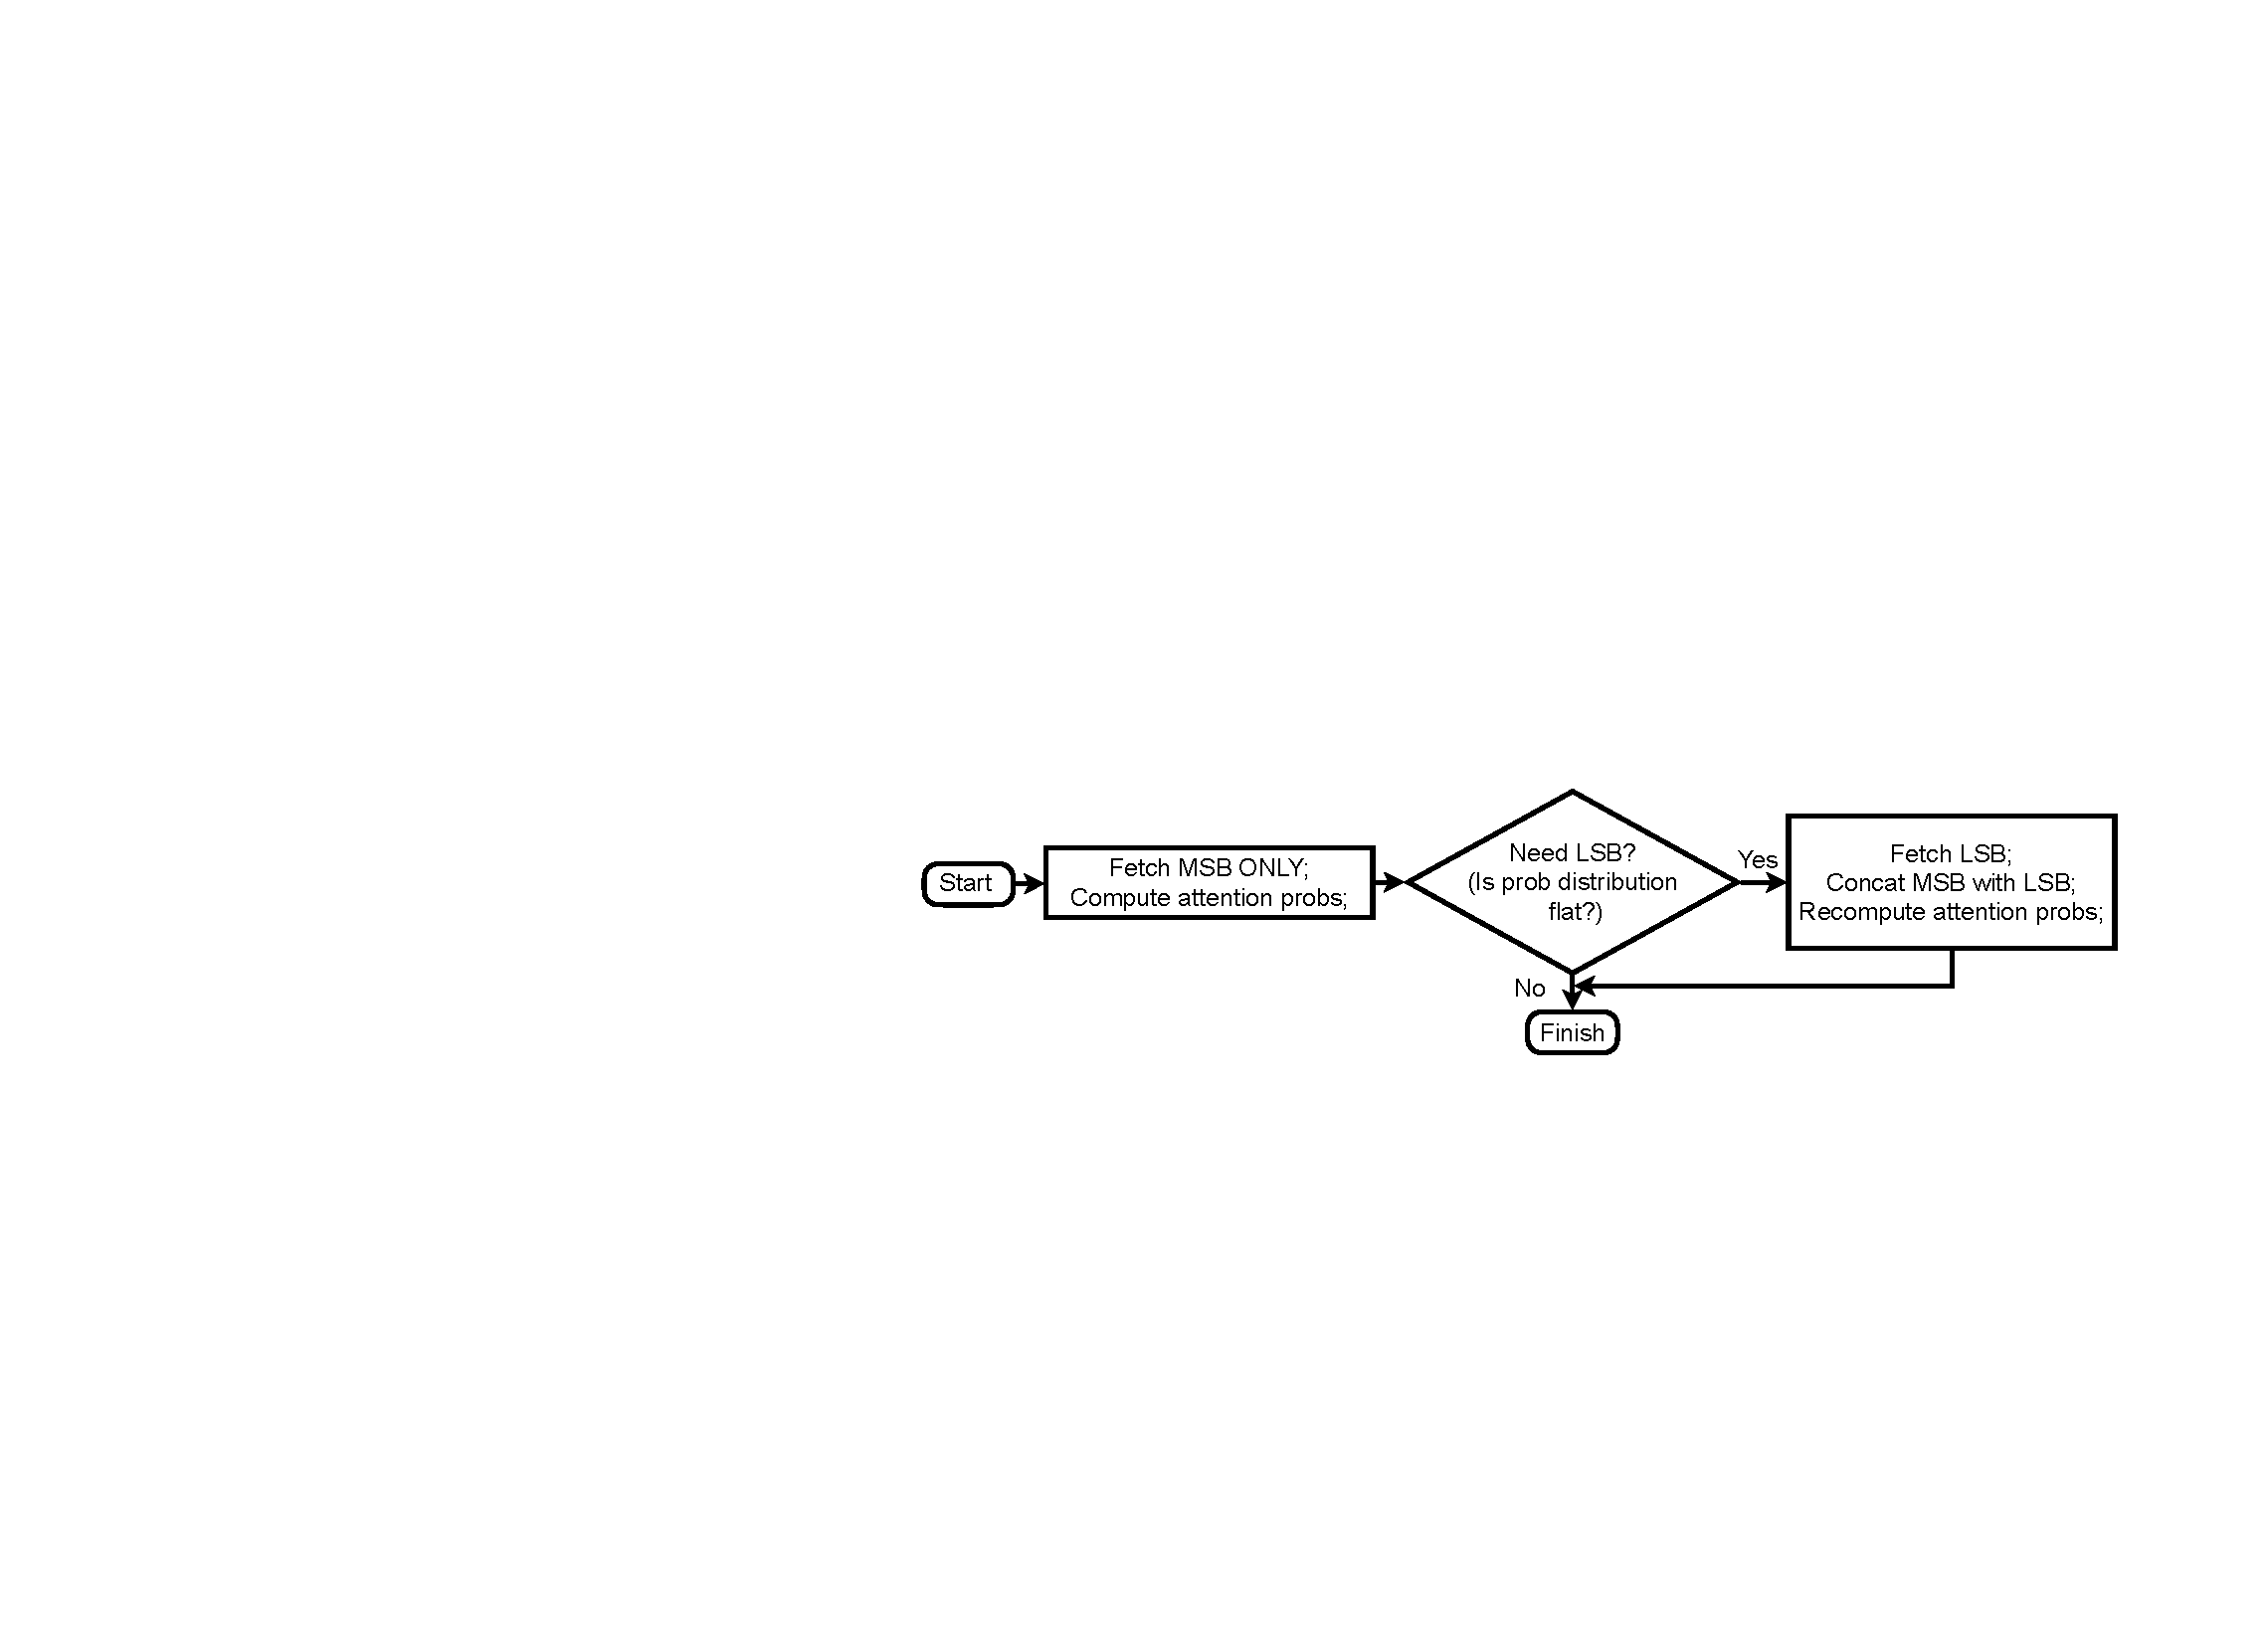
\includegraphics[width=1\columnwidth]{figures/pq_flow.pdf}
    \vspace{-20pt}
    \caption{Progressive Quantization. MSBs are fetched first. Only if the resulting probability distribution is flat, LSBs are fetched, and attention probabilities are recomputed -- this trades computation for memory saving. 
    }
    \vspace{-10pt}
    \label{fig:pq_flow}
\end{figure}

\subsection{Local Value Pruning}
\name also supports local Value (V) pruning, which is performed after \softmax. the V vectors to be pruned are decided \emph{solely with the current head's attention probabilities.} A pre-defined ratio of V vectors with the smallest attention probabilities are pruned and will not be fetched for the $attention\_prob \times$V computation.
Compared to cascade token pruning which removes Q, K, and V of pruned tokens for current and all following attention heads and layers, local V pruning only removes V vectors of the current head.

\subsection{Progressive Quantization}
\label{sec:method:dyna}
\softmax layers are abundant in attention, which allows us to apply more aggressive \lowprec than CNN/RNN models because \softmax can reduce quantization error. Softmax for attention probabilities is:
$p_{i} = e^{s_{i}} / \sum_{j=0}^{L_1-1} e^{s_{j}} $, 
where $L_1$ is the number of K vectors, $p$ is attention probability, and $s$ is attention score. Quantization on Q and K can be considered as adding a small error $\Delta s$ to the attention score $s$. We examine the influence of $\Delta s$ on output attention probabilities by computing the softmax derivative:
\begin{equation}
\label{equ:dsoftmax}
\begin{aligned}
    \mathrm{If \ } i = j: \frac{\partial{p_i}}{\partial{s_j}}
    & = \frac{\partial{\frac{e^{s_{i}}}{\sum_{i=0}^{L_1-1} e^{s_{i}}}}}{\partial{s_i}}
    = p_i \cdot (1-p_i) \\
    \mathrm{If \ } i \neq j: \frac{\partial{p_i}}{\partial{s_j}}
    & = \frac{\partial{\frac{e^{s_{i}}}{\sum_{i=0}^{L_1-1} e^{s_{i}}}}}{\partial{s_j}} 
    = -p_i \cdot p_j
\end{aligned}
\end{equation}
 Without loss of generality, we assume $s_0$ changes by $\Delta s_0 > 0$, and sum the absolute errors of all output with Equation~\ref{equ:dsoftmax}:
\begin{equation}
\label{equ:error}
\begin{aligned}
error 
& = \lvert \Delta s_0 \cdot p_0 \cdot(1-p_0)  \rvert + \sum_{i=1}^{L_1-1} \lvert - \Delta s_0 \cdot p_0 \cdot p_i \rvert \\
& = \Delta s_0 \cdot (2\cdot p_0 \cdot (1-p_0)) < \Delta s_0
\end{aligned}
\end{equation}
Since $0 \le p_0 \le 1$, $2 p_0  (1-p_0)$ is always smaller than 0.5, so the total quantization error is reduced after \softmax.

\begin{figure}[t]
    \centering
    \includegraphics[width=1\columnwidth]{figures/dynamic_precision.pdf}
    \vspace{-20pt}
    \caption{When the attention probability is evenly distributed (left), the quantization error is large; both MSB and LSB are required. When dominant probability exists (right), the quantization error is small; only MSB is required. Grey tokens are pruned by token pruning, thus no need to compute their attention probabilities.
}
    \vspace{-10pt}
    \label{fig:dynamic_precision}
\end{figure}

\begin{figure*}[t]
    \centering
    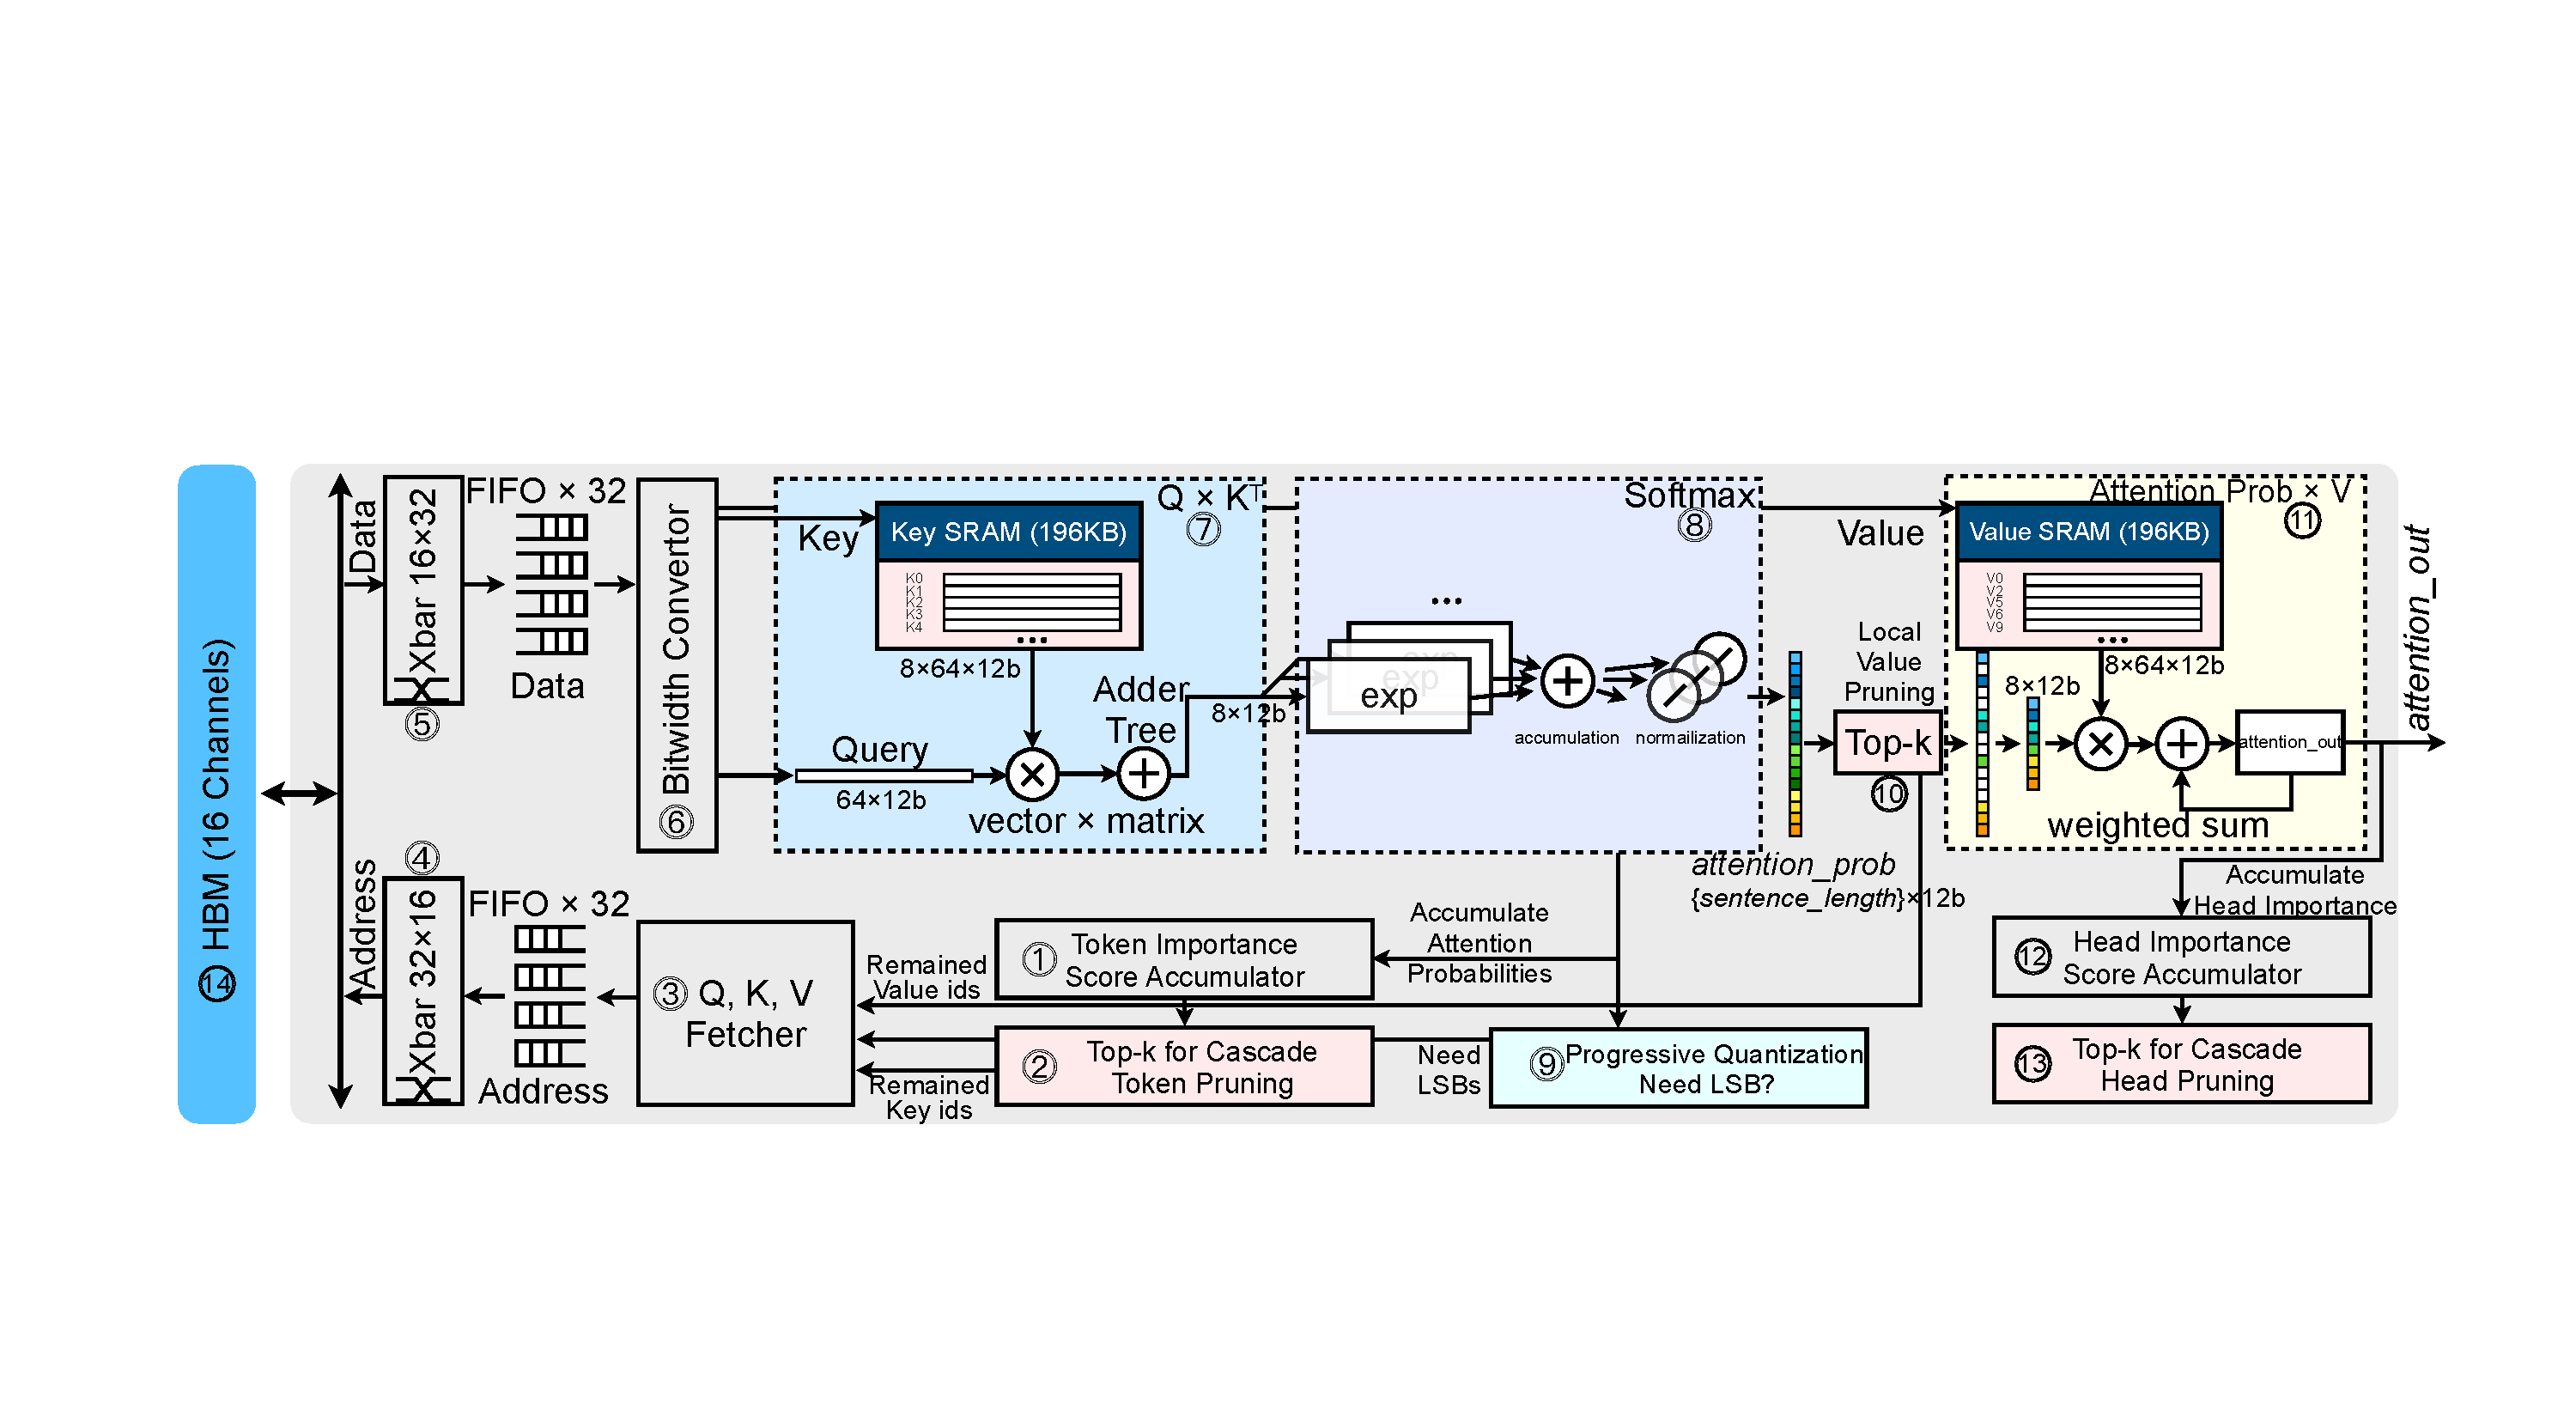
\includegraphics[width=1\textwidth]{figures/arch_overview_new.pdf}
    \vspace{-20pt}
    \caption{SpAtten Architecture Overview. Modules on the critical path (6,7,8,10,11) are fully pipelined to maximize the throughput.}
    \vspace{-10pt}
    \label{fig:arch_overview}
\end{figure*}

On top of static \lowprec, we propose \emph{progressive \lowprec} (Figure~\ref{fig:pq_flow}) to progressively increase the input \bitwidth if aggressive quantization hurts accuracy. An interesting phenomenon in Figure~\ref{fig:dynamic_precision} shows that if the attention probability distribution is dominated by a few tokens, then the 4-bit quantization error is smaller; if flat, the error is larger. Intuitively, dominant tokens are semantically important; thus cannot be easily influenced by quantization. Theoretically, errors are proportional to $p(1-p)$ (Equation~\ref{equ:error}). When probability dominators exist, $p$ is closer to zero or one; thus errors are smaller. Otherwise, errors are larger.
Therefore, for robust layers with probability dominators, the \bitwidth can be small; while other sensitive layers should have more bits. In Figure~\ref{fig:pq_flow}, we firstly apply an aggressive \bitwidth (only fetch MSBs) for inputs and compute the attention probabilities. If the max of computed probability is smaller than a threshold, indicating the distribution is flat, we will fetch LSBs for inputs and recompute the attention probabilities for once. Otherwise, LSBs are not needed. Intuitively, progressive quantization finds which input sample is \emph{more difficult} and applies a higher bitwidth instead of using a high bitwidth universally, thus reducing DRAM access under the same accuracy.

For fast interactions between \name and hardware for FC parts, we conduct \emph{linear symmetric quantization}, which is much faster than K-Means quantization. We have five different MSB+LSB settings: 4+4, 6+4, 8+4, 10+4, and 12+4. The settings can be different across tasks but are the same within one task. Different inputs of one task determine \emph{whether to fetch LSB on the fly}. We store MSBs continuously and LSBs continuously in DRAM, so that they can be fetched separately.
Progressive \lowprec trades more computation for less memory access and can effectively accelerate memory-bounded generative models such as \gpttwo. It also improves energy efficiency since DRAM access takes around 70\% of \name power, much expensive than computation.  
On average, only 5.9\% input samples require LSB. For \bert, we only apply static quantization because \bert models are computation-bounded, and fetching LSB for recomputation will degrade \bert's performance.
